As it  has been detailed during all the memory of the master's thesis that the process of training a model essentially revolves around the optimization of a particular function. Essentially, the suitable loss function is not only hard to come up but also it might be impossible since any function has their payoff. In this section, a review of the metrics and losses will be carried out to understand their advantages and disadvantages when applying them. However, those function loss described before such as the \gls{gan} (equation \ref{eq:gan}), \gls{vae} (equation \ref{eq:vae}) or \gls{ddm} (equation \ref{eq:ddm}) losses.
\\\\
The \gls{mse} Mean Squarred Error loss computes the mean of the squared differences between the target values and the predicted values. It is the most common used when using autoencoders. It is given by
\[MSE(y, \hat{y}) = \frac{1}{n} \sum_{i=1}^{n}(y_i - \hat{y}_i)^2\]
One of the main advantages of this loss is that squaring the differences magnifies the errors, making the model more sensitive to data points that are far from the predicted values. It is also often used in regression problems and highly sensitive to outliers due to the squarring term. However, when it comes to generative image models, this loss tend to produce some noise in the synthetic images.
\\\\
The L1 loss or \gls{mae} Mean Absolute Error loss computes the mean of the absolute differences between the target values and the predicted values. It is used when aiming to reduce the noise from the output image. It is given by
\[L1(y, \hat{y}) = \frac{1}{n} \sum_{i=1}^{n}|y_i-\hat{y_i}|\]
It is less sensitive to outliers compared to \gls{mse} loss because it doesn't square the differences. 
\\
\\
The \gls{sam} is a widely used algorithm for comparing spectral similarity between two spectra. It calculates the angle between two spectra, treating them as vectors in a space with as many dimensions as there are bands. The smaller the angle, the more similar the two spectra.
\[SAM(y, \hat{y}) = \arccos (\frac{y \times \hat{y}}{||y|| \cdot ||\hat{y}||})\]

A loss or metric used only in cloud removal state of the art is the \gls{carl}. It is a custom loss function, typically used when there is the cloud mask. This loss function is constructed to handle areas in satellite images that are clear or cloudy differently. This metric focuses on minimizing the differences between the clear regions of the input image and the synthetic image. For that reason, for clear regions, it is used the \gls{mae} between the output and the input image, and, for cloudy images, it is used the \gls{mae} between the output and the target image. Additionally, there's a penalty term added to the loss which is simply the mean absolute error between the predicted values and the true target values, weighted by a factor. Normally, $w = 1$.
\begin{align*}
	CARL(x, y, \hat{y}, mask_{cloud}) =& \quad  \frac{\sum_{i=1}^{n} (A - mask_{cloud}) \times |(x_i - \hat{y_i})|}{n} \, + \\  & \quad + \frac{\sum_{i=1}^{n} mask_{cloud} \times |(y_i - \hat{y_i})|}{n} \, + \\ & \quad + w \cdot \frac{\sum_{i=1}^{n} |y_i - \hat{y_i}| }{n}
\end{align*}
\[\text{being} \quad A = 
\begin{pmatrix}
	1 & 1 & ... & 1 \\
	1 & 1 & ... & 1 \\
	... & ... & ... & ... \\
	1 & 1 & ... & 1
\end{pmatrix}\\
\quad\\\]
In essence, the \gls{carl} loss aims to:
\begin{itemize}
	\item Penalize large differences in clear areas between predictions and cloudy inputs.
	\item Penalize large differences in cloudy or shadowed areas between predictions and true values.
	\item Apply an overall penalty for differences between predictions and true values across the entire image.
\end{itemize}
Normally, no classifications loss functions would be used in generative models. Although, since \gls{gan}s, more specifically, discriminators, need to discern between real and fake images, it is notable to mention the \gls{bce} loss, whcih, actually, is regularly used in binary classification. A grosso modo \gls{bce} calculates the dissimilarity between the true distribution of labels and the predicted probability distribution. In other words, it doesn't just look at the raw value of the prediction but considers it as a probability distribution. 
\[BCE(x, y) = -(y \cdot log(x) + (1 - y) \cdot log (1 - x))\]
A lower \gls{bce} indicates that the predicted probabilities are closer to the true labels, while a higher \gls{bce} suggests a larger discrepancy. Since it is measuring probabilities, it is compulsary to output a value between 0 and 1. 
\\
\\
When referring to image processing and computer vision, there are metrics to measure the similarity between two images. The \gls{psnr} is a metric commonly used to measure the quality of reconstructed or compressed images in comparison to a reference image. It is particularly popular in the fields of image and video compression, as it gives an objective measure of the reconstruction quality. The \gls{psnr} is derived from the \gls{mse} between the reference and the reconstructed image.
\[PSNR(y, \hat{y}) = 10 \cdot log_{10} \frac{(MAX_I^2)}{MSE(y, \hat{y})}\]
where $MAX_I$ is the maximum possible pixel value of the image, in our case, 1. The PSNR is usually expressed in decibels (dB). A higher PSNR indicates better reconstruction quality, implying that the reconstructed image is closer to the reference image. Conversely, a lower PSNR suggests that the image quality has deteriorated. It's worth noting that while PSNR is a straightforward and widely-used metric, it doesn't always align perfectly with human perception. In some cases, images with higher PSNR may appear of lower quality to human viewers, and vice-versa. 
\\
\\
Another metric used in image processing is the \gls{ssim}. It was developed to provide a more intuitive quality metric than traditional methods like \gls{mse} or \gls{psnr}. While \gls{mse} and \gls{psnr} are based on pixel-wise differences, \gls{ssim} considers changes in structural information, luminance, and texture.\\
\\
The SSIM index is defined for two windows $x \in \text{img}_1$ and $y \in \text{img}_1$.  The formula for \gls{ssim} is given by:
\[SSIM(x, y) = \frac{(2 \mu_x \mu_y + C_1)(2 \sigma_{xy} + C_2)}{(\mu_x^2 + \mu_y^2 + C_1) (\sigma_x^2 + \sigma_y^2 + C_2)}\]
where:
\begin{itemize}
	\item $\mu_x$ and $\mu_y$ are the average values for windows $x$ and $y$ respectively.
	\item $\sigma_x^2$ and $\sigma_y^2$ are the variances of windows $x$ and $y$ respectively.
	\item $\sigma_xy$ is the covariance between both windows.
	\item $C_1$ and $C_2$ are constants to stabilize the division against weak denominators. They are typically set as $C_1 = (k_1L)^2$ and $C_2 = (k_2L)^2$ where $L$ is the range of the pixel values. In our case, $L = 1$. On the other hand, $k_1$ and $k_2$ are small constants, which are commonly set to $k_1=0.01$ and $k_2=0.03$. 
\end{itemize}
The \gls{ssim} index can be computed for every window in the image, and the results can be averaged to produce a single SSIM value for the entire image. If the valuyes of the metric is $1$, it indicates that the two images are identical, being the upper bound of the index. Values further than 1 indicate less similarity.
\begin{figure}[H]
	\centering
	\begin{adjustwidth}{-5cm}{}
		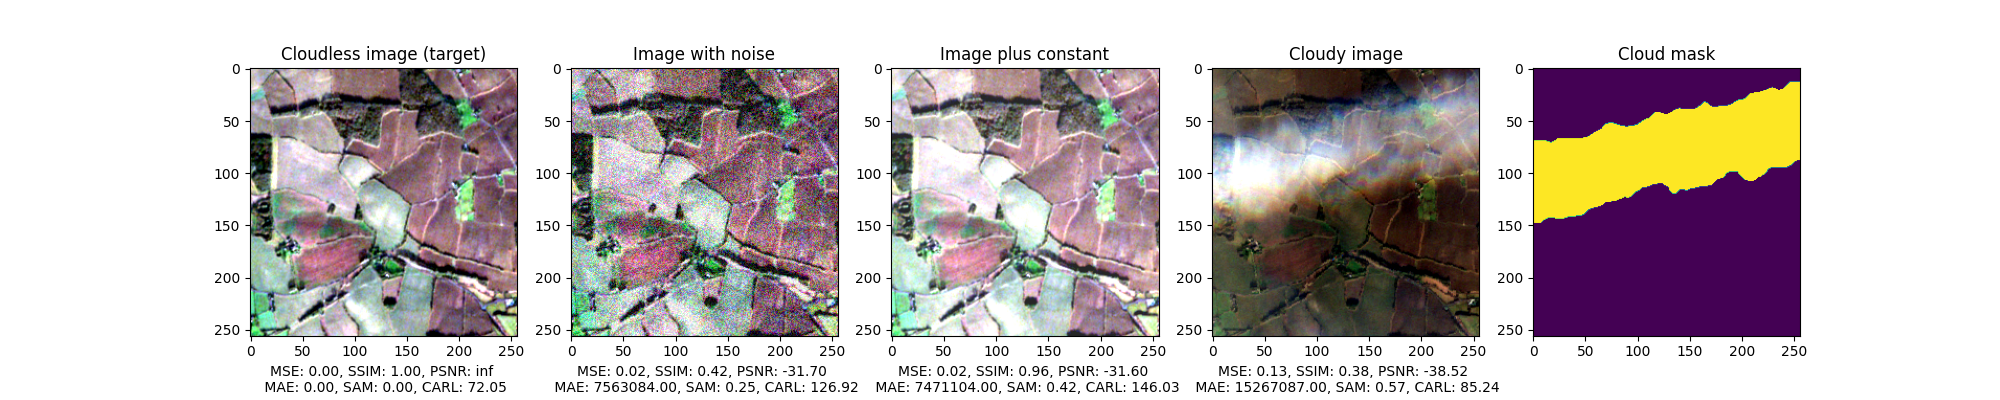
\includegraphics[width=24cm]{imgs/models/metrics/approach}
	\end{adjustwidth}
	\caption{Comparison of all the metrics ($w=1$).}
	\label{fig:models-metrics-comparison}
\end{figure}
To sum up, it has been done a comparison of these metrics between a cloudy and a cloudless image. To help the comparison, it has modified the cloudless image to create two possible outputs from the model: one with noise and one adding a constant. In that case, it is notable that \gls{ssim} puts more attention to the structural information and \gls{mse}, \gls{sam} or \gls{carl} check pixel-wise differences. It is worth noting how \gls{carl} benefits cloudy images than those who are modified. That is because this function depends on the cloud mask and how different are the cloudless and the cloudy image. Taking that into account, \gls{carl} needs to be used more like a loss function, where the model would try to optimize not only the cloud removal but also the minimum differences in clear regions than a metric to check how good is the model trying to remove the clouds without considering its consequences. Nevertheless, we must take into consideration that the intensity values from the pixels are from 0 to 256, if they were normalized, \gls{carl} results would be between $[0, (2 + w)]$.
\begin{table}[H]
	\caption{Comparison of all the metrics.}
	\begin{tabular}{l|cccccc}
		Image & MSE & SSIM & PSNR & MAE & SAM & CARL(w=1)\\\hline
		Cloudless (target) & 0 & 1 & inf & 0 & 0 & 72.05\\
		Noisy image & 0.02 & 0.42 &  -31.70 & 7563250 & 0.25 & 126.92\\
		Image plus constant & 0.02 & 0.96 & -31.60 & 7471104 & 0.42 & 146.03\\
		Cloudy image & 0.13 & 0.38 & -38.52 & 15267087 & 0.57 & 85.24\\
	\end{tabular}
\end{table}

